% !TeX TXS-program:compile = txs:///arara
% arara: lualatex: {shell: no, synctex: yes, interaction: batchmode}
% arara: lualatex: {shell: no, synctex: yes, interaction: batchmode} if found('log', '(undefined references|Please rerun|Rerun to get)')

\documentclass[a4paper]{scrartcl}
\usepackage{mathtools, array, varioref}
\usepackage[british]{babel}
\usepackage{pennstander-otf}
\usepackage{framed}
\usepackage{unicodefonttable}
\usepackage{realscripts}
\usepackage{graphicx}
\renewcommand{\sffamily}{\rmfamily}
\setmonofont{CascadiaMono}[Scale=MatchLowercase]
\usepackage{subfig}
\captionsetup[subtable]{position=top}
\usepackage{fourier-orns}
\usepackage{microtype}

\newcommand*{\pkg}[1]{\texttt{#1}}
\newcommand*{\file}[1]{\texttt{#1}}
\newcommand*{\ttbold}[1]{\texttt{\textbf{#1}}}
\newcommand*{\opt}[1]{\texttt{#1}}
\newcommand*{\cmd}[1]{\texttt{\textbackslash #1}}\newcommand*{\showtchar}[1]{\cmd{#1}~\csname #1\endcsname}
\newcommand*{\showmchar}[1]{\cmd{#1}~$(\csname #1\endcsname)$}
\newcommand*{\showmchardollar}[1]{\texttt{\$\cmd{#1}\$}~$(\csname #1\endcsname)$}

%\renewcommand{\labelitemi}{\lefthand}

\newcommand{\abc}{abcdefghijklmnopqrstuvwxyz}
\newcommand{\ABC}{ABCDEFGHIJKLMNOPQRSTUVWXYZ}
\newcommand{\samplenumbers}{0123456789}

%\usepackage{setspace}
%\setstretch{1.20}
\setlength{\parindent}{0pt}
%\setlength{\parskip}{12pt plus 3pt minus 3pt}
\setlength{\parskip}{6pt plus 2pt minus 2pt}

\usepackage{hyperref}
\hypersetup{pdftitle={Pennstander User’s Guide for LaTeX},
	pdfauthor={Cédric PIERQUET},
	bookmarksopen,
	colorlinks
}
\newcommand*{\hlabel}[1]{\phantomsection\label{#1}}

\title{Pennstander fonts (\textit{experimental}) \\User’s Guide for LaTeX}
\author{Julius Ross \&\ Cédric Pierquet \\ \texttt{cpierquet@outlook.fr}}

\date{\today}
\newcommand*{\version}{0.3}
%\newif\ifCTAN   \CTANtrue  %%% décommenter pour CTAN


\begin{document}
\maketitle

\section{What is Pennstander ?}

Pennstander is a set of OpenType text and math fonts developed by Julius Ross, see \url{github.com/juliusross1} for more information.

The text and the math fonts are licensed under the SIL Open Font License, Version 1.1.

They require LuaTeX or XeTeX as engine and the \pkg{unicode-math} package\footnote{Please read the documentation \file{unicode-math.pdf}.}, if math fonts are required or just the \pkg{fontspec} package\footnote{Please read the documentation \file{fontspec.pdf}.} otherwise.

\section{Usage}

\subsection{Loading text fonts and math fonts}

Several weights are available:

\hfill\opt{Thin / ExtraLight / Light / Regular / Medium / SemiBold / Bold}\hfill\null

for text or math version.

\smallskip

Files \file{Pennstander(math)-<weight>.fontspec} are provided to ensure that Italic, Bold, BoldItalic ans (fake)Slanted variants are properly loaded.

\smallskip

A basic call for Pennstander text and math fonts with scaling could be:

\begin{verbatim}
\usepackage{pennstander-otf}
\end{verbatim}

It loads:

\begin{itemize}
	\item \opt{Pennstander-Regular} as main font;
	\item \opt{PennstanderMath-Regular} as math font.
\end{itemize}

It defines \cmd{eff} for \textit{florin math} $\eff$.

\begin{oframed}
\textbf{Theorem 1 (Residue Theorem).}
Let $f$ be analytic in the region $G$ except for the isolated singularities $a_1,a_2,\ldots,a_m$. If $\gamma$ is a closed rectifiable curve in $G$ which does not pass through any of the points $a_k$ and if $\gamma\approx 0$ in $G$ then
\[
\frac{1}{2\pi i}\int_\gamma f = \sum_{k=1}^m n(\gamma;a_k) \text{Res}(f;a_k).
\]

\textbf{Theorem 2 (Maximum Modulus).}
\emph{Let $G$ be a bounded open set in $\mathbb{C}$ and suppose that $f$ is a continuous function on $G^-$ which is analytic in $G$. Then}
\[
\max\{|\eff(z)|:z\in G^-\}=\max \{|\eff(z)|:z\in \partial G \}.
\]
\end{oframed}

\subsection{Options}

Options can be given within the package:

\begin{itemize}
	\item \opt{Weight=...}, within \opt{Thin/ExtraLight/Light/Regular/Medium/SemiBold/Bold};
	\item the boolean \opt{no-text} fot not loading pennstander as main font;
	\item the boolean \opt{no-math} fot not loading pennstander as math font;
	\item \opt{math-style=...} for unicode-math option;
	\item \opt{bold-style=...} for unicode-math option;
	\item \opt{StylisticSet=...}
	\item \opt{RawFeatureT=...} for text version;
	\item \opt{RawFeatureM=...} for math version;
	\item \opt{Scale=...}
\end{itemize}

\subsection{Manual loading}

It's also possible to load text and/or math fonts with \cmd{setmainfont} and/or \cmd{setmathfont}, thanks to \opt{fontspec} files for example.

\begin{verbatim}
%w/o package loaded
\usepackage{fontspec}
\usepackage{unicode-math}
\setmainfont{Pennstander-<weight>}[options]
\setmainfont{PennstanderMath-<weight>}[options]
\end{verbatim}

\section{Openfeatures}

\subsection{For text font}

Extra openfeatures for text font available are (screens are from fontdrop website):

\begin{itemize}
	\item \opt{aalt}: Access All Alternatives
	\item \opt{ccmp}: Glyph Composition/Decomposition
	\item \opt{locl}: Localized Forms
	\item \opt{sups}: Superscript
	\item \opt{numr}: Numerators
	\item \opt{dnom}: Denominators
	\item \opt{frac}: Fractions
	\item \opt{ordn}: Ordinals
	\item \opt{pnum}: Proportional Figures
	\item \opt{tnum}: Tabular Figures
	\item \opt{case}: Case-Sensitive Forms
	\item \opt{dlig}: Discretionary Ligatures
	\item \opt{liga}: Standard Ligatures
	\item \opt{zero}: Slashed Zero
	\item \opt{cpsp}: Capital Spacing
	\item \opt{ss02}: Alternate A,M,N,Q,V,W,Z,v,z
	\item \opt{ss03}: Alternate 4
	\item \opt{ss04}: Alternate l,t
	\item \opt{ss06}: Alternate ampersand
	\item \opt{ss07}: Alternate 7
\end{itemize}

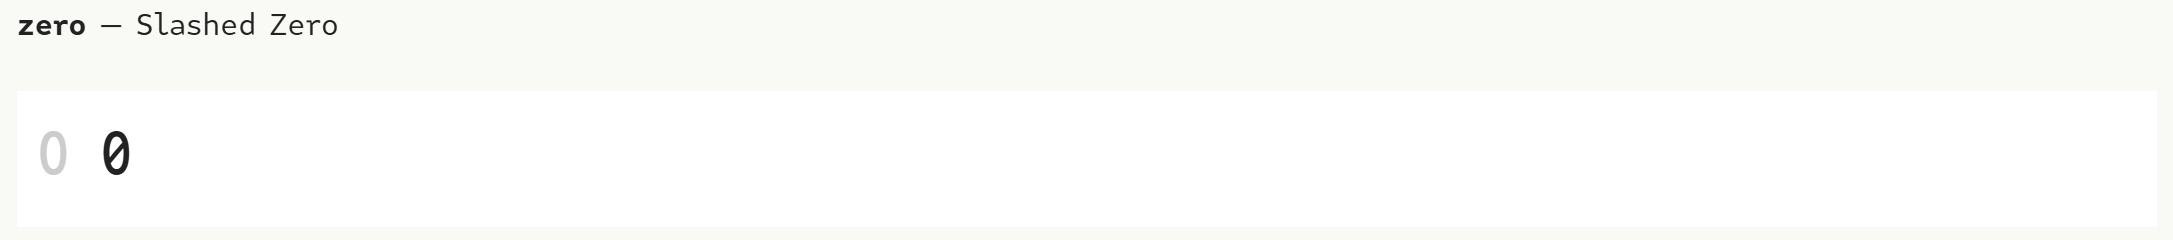
\includegraphics[width=0.525\linewidth]{pennstander_zero}

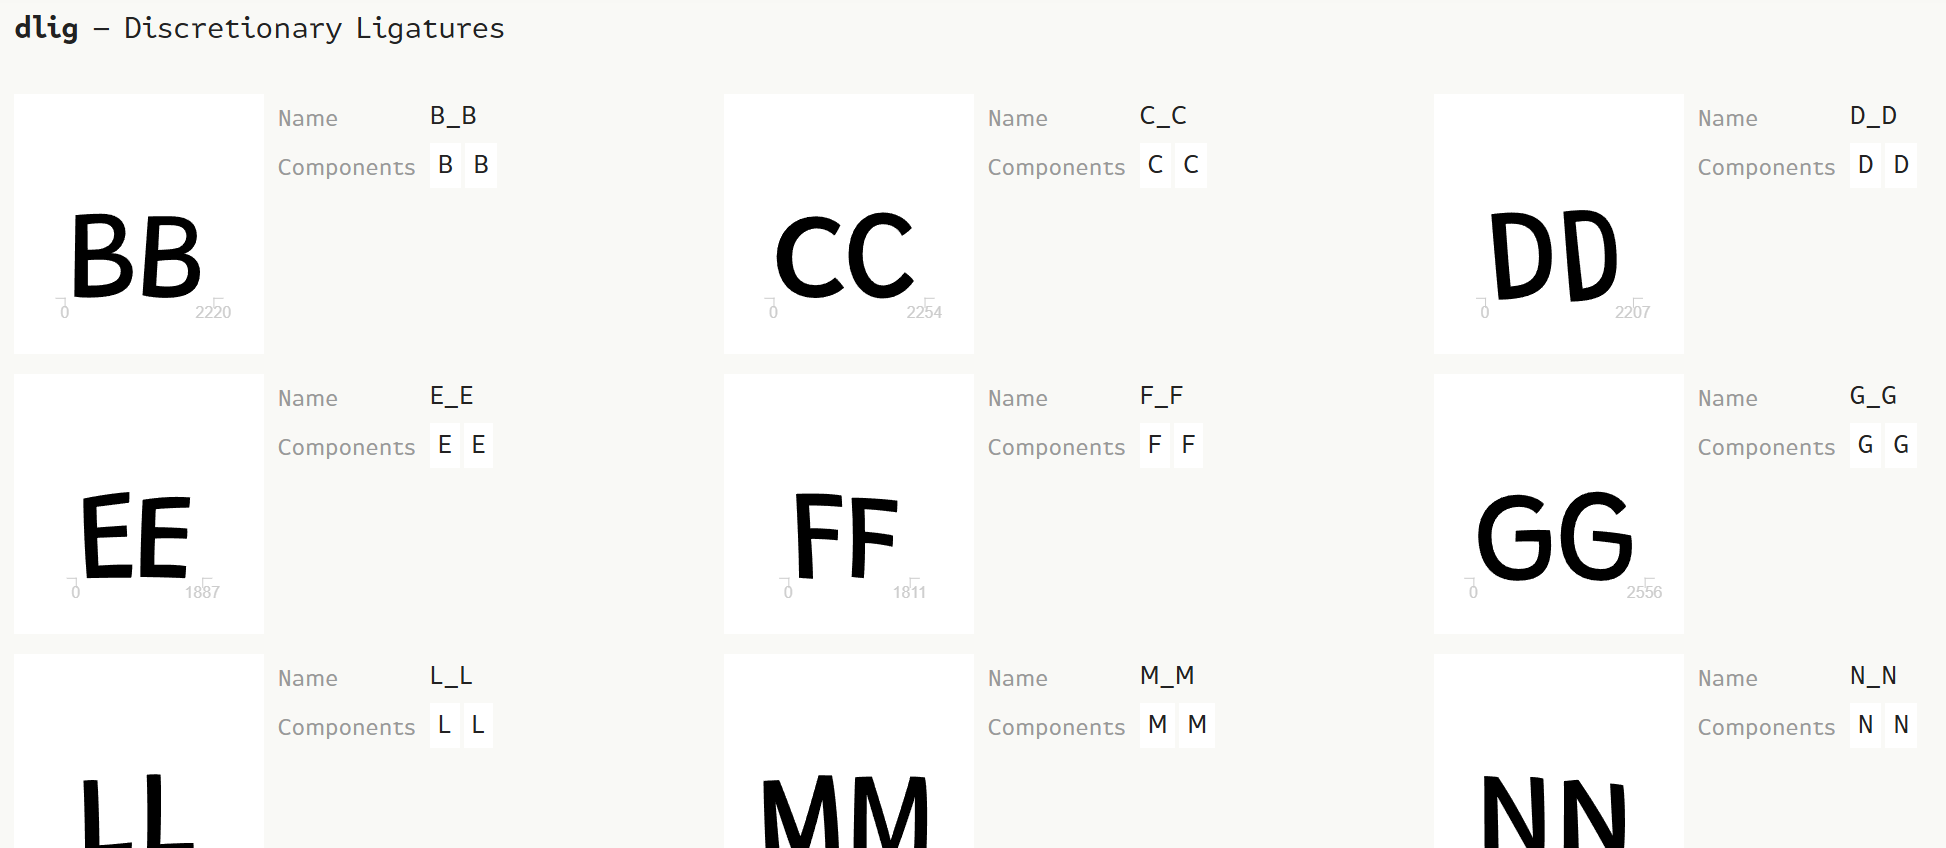
\includegraphics[width=0.525\linewidth]{pennstander_dlig}

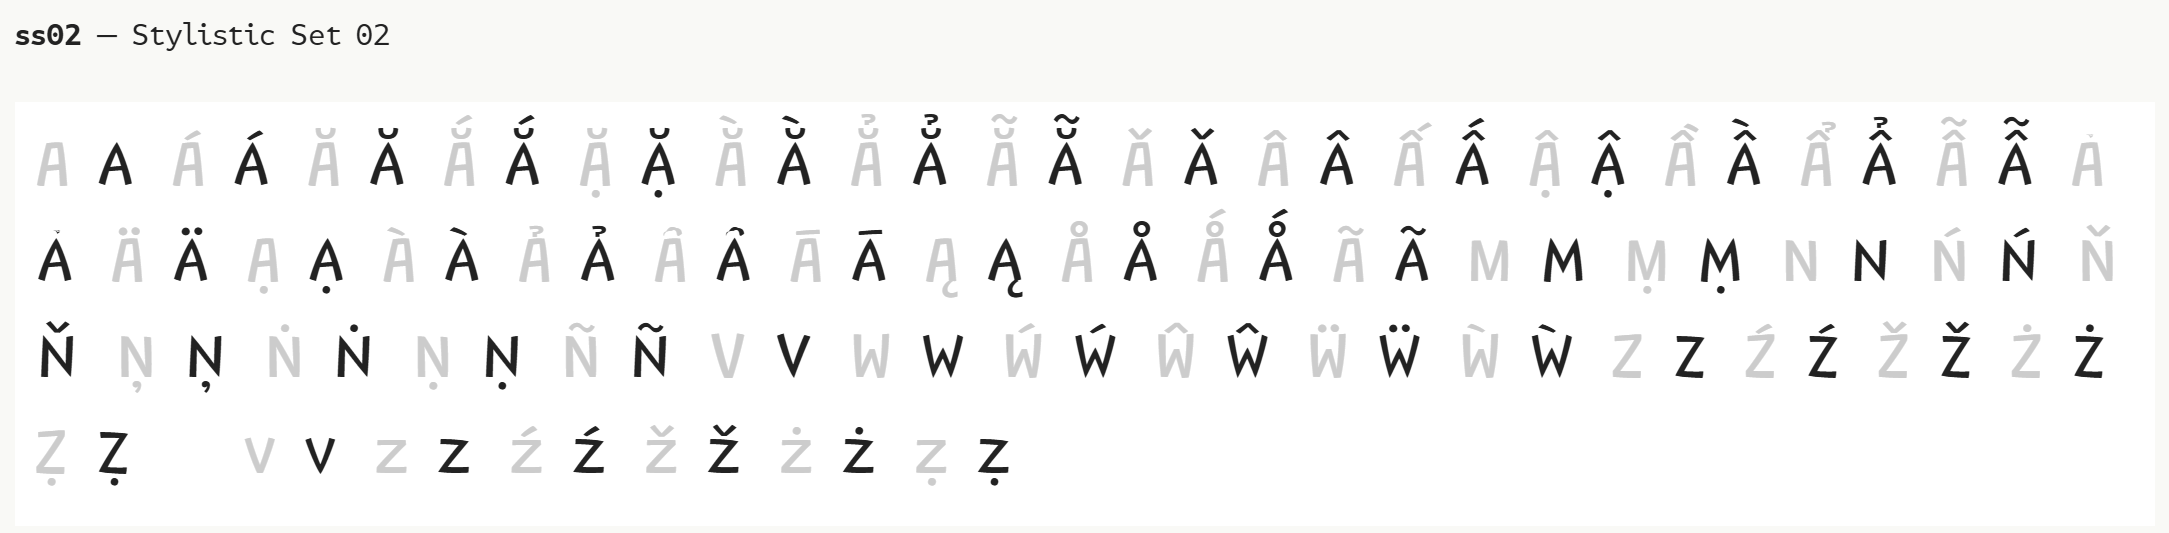
\includegraphics[width=0.525\linewidth]{pennstander_ss02}

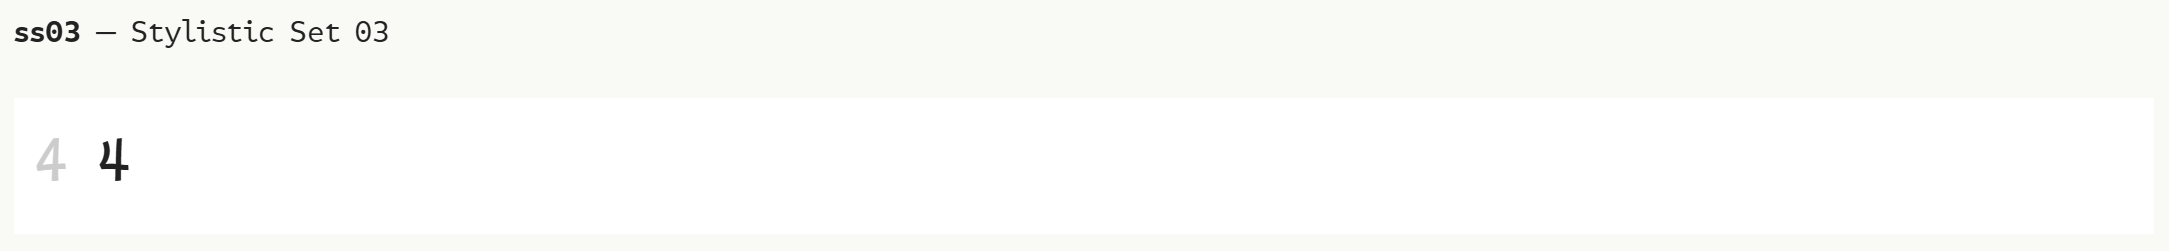
\includegraphics[width=0.525\linewidth]{pennstander_ss03}

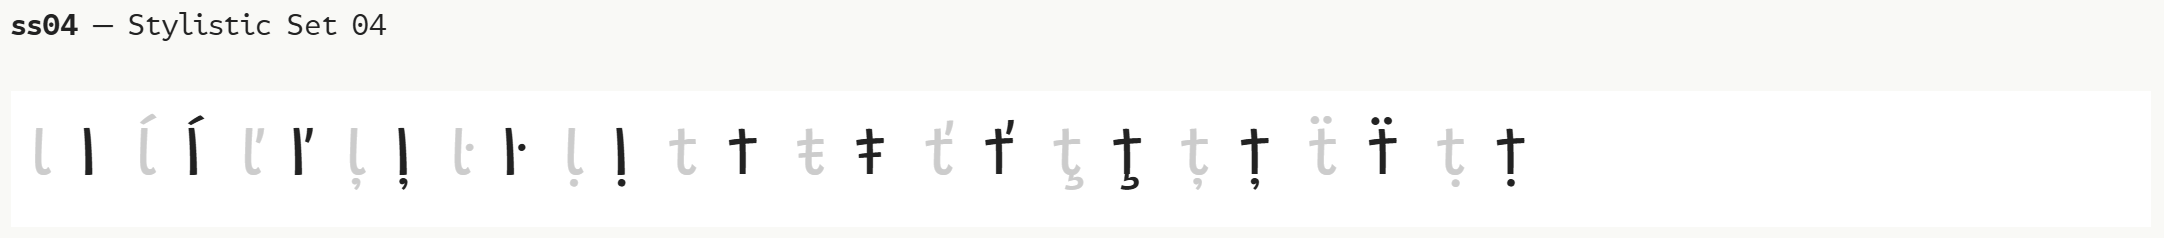
\includegraphics[width=0.525\linewidth]{pennstander_ss04}

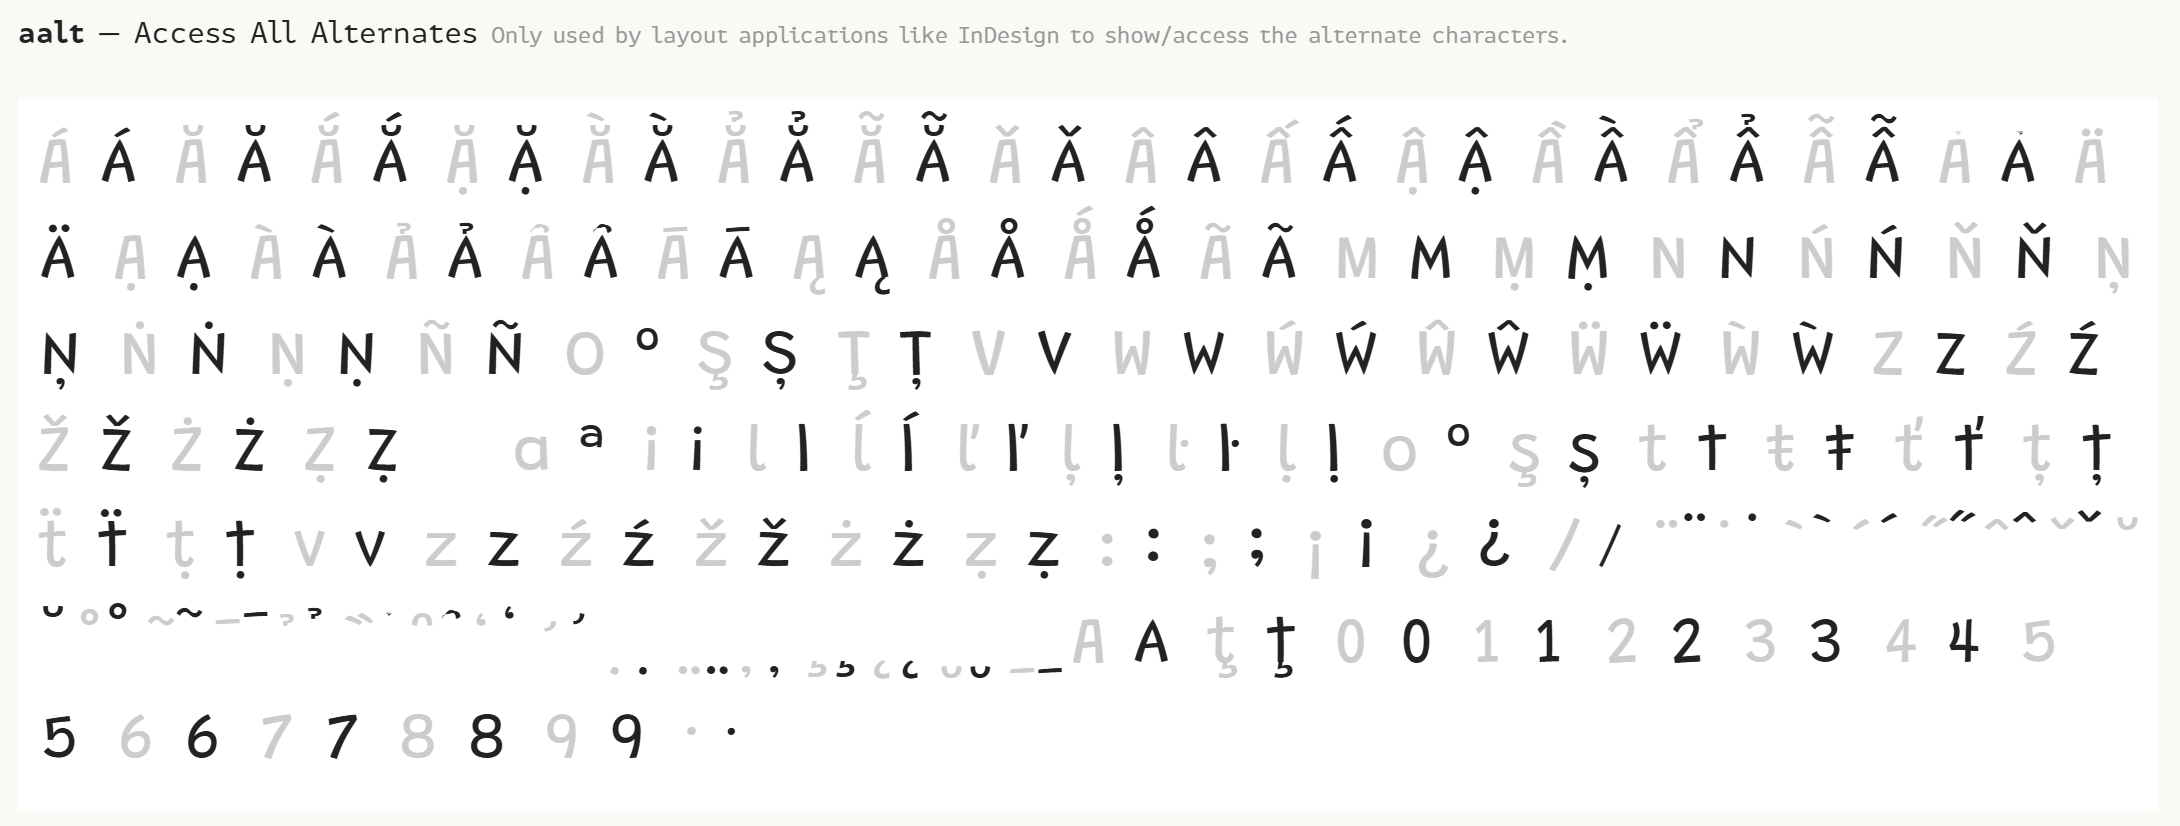
\includegraphics[width=0.525\linewidth]{pennstander_aalt}

\subsection{For math font}

Extra openfeatures for math font available are:

\begin{itemize}
	\item \opt{aalt}: Access All Alternatives
	\item \opt{dtls}: Dotless Forms
	\item \opt{zero}: Slashed Zero
	\item \opt{frac}: Fractions
	\item \opt{ss01}: Alternate a,g,I,Iota
	\item \opt{ss02}: Alternate A,M,N,Q,V,W,Z,v,z,Alpha,Mu,Rho,Zeta
	\item \opt{ss03}: Alternate 4
	\item \opt{ss04}: Alternate l,t
	\item \opt{ss05}: Simplified Fraktur A,K,L,X,Y,Z,x,y
	\item \opt{ss07}: Alternate 7
\end{itemize}

\subsection{Unicode Private Use Area}

Glyphs assigned to Unicode Private Use Area:

\begin{itemize}
	\item Double-struck uppercase Greek letters: \opt{U+E1002–U+E1008}
	\item Fraction Rule: \opt{U+E000}
	\item Radical Rule: \opt{U+E001}
\end{itemize}

\section{List of glyphs}

\subsection{Text version}

\displayfonttable{Pennstander-Regular}

\subsection{Math version}

\displayfonttable{PennstanderMath-Regular}

\section{Alphabets}

\subsection{Text version}

-- Normal/\textbf{Bold}/\textit{Italic}/\textit{\textbf{BoldItalic}}/\textsl{Slanted}/\textsl{\textbf{BoldSlanted}}:

\abc\ABC\samplenumbers

\textbf{\abc\ABC\samplenumbers}

\textit{\abc\ABC\samplenumbers}

\textit{\textbf{\abc\ABC\samplenumbers}}

\textsl{\abc\ABC\samplenumbers}

\textsl{\textbf{\abc\ABC\samplenumbers}}

\smallskip

\textit{Slanted version are \textbf{FakeSlanted} with 0.19 coefficient.}

\subsection{Math version}

-- Normal/\textbf{Bold}/\textit{Italic}/\textit{\textbf{BoldItalic}}:

$\abc\ABC\samplenumbers$

$\mathbf{\abc\ABC\samplenumbers}$

$\mathit{\abc\ABC\samplenumbers}$

$\mathit{\mathbf{\abc\ABC\samplenumbers}}$

\smallskip

-- mathcal/mathfrak/mathbb:

$\mathcal{\abc\ABC}$

$\mathfrak{\abc\ABC}$

$\mathbb{\ABC\samplenumbers}$
%\section{What is provided by Luciole-Math?}
%
%Luciole-Math provides a wide range of glyphs including all those available in
%the \pkg{amssymb} and \pkg{latexsym} packages.  Therefore,
%the latter two packages \emph{should not} be loaded as they might override
%Luciole-Math glyphs.
%
%A full list of available glyphs is shown in file \file{unimath-luciole.pdf}.
%
%\subsection{Upright or slanted?}
%\label{ssection-um}
%
%Package \pkg{unicode-math} follows \TeX{} conventions for Latin and Greek
%letters: in math mode, the default option (\opt{math-style=TeX}) prints
%Latin letters $a$…$z$ $A$…$Z$ and lowercase Greek letters $\alpha$…$\omega$
%slanted (italic) while uppercase Greek letters $\Alpha \Beta \Gamma$…$\Omega$
%are printed upright.
%This can be changed by option \opt{math-style} as shown in
%table~\vref{math-style}.
%
%\begin{table}[ht]
%	\centering
%	\caption{Effects of the \opt{math-style} package option.}
%	\hlabel{math-style}
%	\begin{tabular}{@{}>{\ttfamily}lcc@{}}
%		\hline
%		\rmfamily Package option & Latin & Greek \\
%		\hline
%		math-style=ISO & $(a,z,B,X)$ & $\symit{(\alpha,\beta,\Gamma,\Xi)}$ \\
%		math-style=TeX & $(a,z,B,X)$ & $(\symit\alpha,\symit\beta,\symup\Gamma,\symup\Xi)$ \\
%		math-style=french & $(a,z,\symup B,\symup X)$ & $(\symup\alpha,\symup\beta,\symup\Gamma,\symup\Xi)$ \\
%		math-style=upright & $(\symup a,\symup z,\symup B,\symup X)$ & $(\symup\alpha,\symup\beta,\symup\Gamma,\symup\Xi)$ \\
%		\hline
%	\end{tabular}
%\end{table}
%
%Bold letters are printed upright except lowercase Greek letters
%which are slanted (the default option is \opt{bold-style=TeX}). This can be
%changed by option \opt{bold-style} as shown in table~\vref{bold-style}.
%
%\begin{table}[ht]
%	\centering
%	\caption{Effects of the \opt{bold-style} package option.}
%	\hlabel{bold-style}
%	\begin{tabular}{@{}>{\ttfamily}lcc@{}}
%		\hline
%		\rmfamily Package option & Latin & Greek \\
%		\hline
%		bold-style=ISO & $(\symbfit a, \symbfit z, \symbfit B, \symbfit X)$ & $(\symbfit\alpha, \symbfit\beta, \symbfit\Gamma, \symbfit\Xi)$ \\
%		bold-style=TeX & $(\symbfup a,\symbfup z,\symbfup B,\symbfup X)$ & $(\symbfit\alpha, \symbfit\beta,\symbfup \Gamma,\symbfup \Xi)$ \\
%		bold-style=upright & $(\symbfup a,\symbfup z,\symbfup B,\symbfup X)$ & $(\symbfup \alpha,\symbfup \beta,\symbfup \Gamma,\symbfup \Xi)$ \\
%		\hline
%	\end{tabular}
%\end{table}
%
%Other possible customisation: $\nabla$ is printed upright and $\partial$ is
%printed slanted by default, but \opt{nabla=italic} and
%\opt{partial=upright} can change this.
%
%All these options are offered by the \pkg{unicode-math} package, they can
%be added to the \cmd{setmathfont} call as well%
%\footnote{IMHO it is easier to add \emph{all options} to the \cmd{setmathfont}
%	command.}, for example:
%
%\verb+\setmathfont{Luciole-Math.otf}[math-style=french,partial=upright]+\\
%will print for the code
%\begin{verbatim}
%	\[ \frac{\partial f}{\partial x} = \alpha \symbf{V}
%	+ a\nabla\Gamma + \symbf{\beta}\symbf{M} \]
%\end{verbatim}
%\setmathfont{Luciole-Math.otf}[math-style=french,partial=upright]
%\[\frac{\partial f}{\partial x} = \alpha \symbf{V} + a\nabla\Gamma +
%\symbf{\beta}\symbf{M} \]
%while the default settings would print
%\setmathfont{Luciole-Math.otf}[math-style=TeX,partial=italic]
%\[\frac{\partial f}{\partial x} = \alpha \symbf{V} + a\nabla\Gamma +
%\symbf{\beta}\symbf{M} \]
%
%Both shapes remain available anytime: \verb+$\uppi,\itpi$+
%prints $\uppi, \itpi$.
%
%If your text editor is able to handle Greek letters or math symbols, they can
%be entered in the code instead control sequences (i.e.
%$\symup{α}$, $\symup{β}$, $\symup{Γ}$,… for \cmd{alpha}, \cmd{beta},
%\cmd{Gamma},…).
%
%\subsection{Character variants}
%\label{ssection-cv}
%
%Luciole-Math provides eleven ``Character Variants'' options, listed on
%table~\vref{cv}.
%
%\begin{table}[ht]
%	\centering  \caption{Character variants.}
%	\hlabel{cv}
%	\begin{tabular}{@{}>{\ttfamily}lccl@{}}
%		\hline
%		& Default       & Variant          & Name\\
%		\hline
%		cv01 & $\hslash$     & $\mithbar$       & \cmd{hslash} \\
%		cv02 & $\emptyset$   & $\varemptyset$   & \cmd{emptyset} \\
%		cv03 & $\epsilon$    & $\varepsilon$    & \cmd{epsilon} \\
%		cv04 & $\kappa$      & $\varkappa$      & \cmd{kappa} \\
%		cv05 & $\pi$         & $\varpi$         & \cmd{pi} \\
%		cv06 & $\phi$        & $\varphi$        & \cmd{phi} \\
%		cv07 & $\rho$        & $\varrho$        & \cmd{rho} \\
%		cv08 & $\sigma$      & $\varsigma$      & \cmd{sigma} \\
%		cv09 & $\theta$      & $\vartheta$      & \cmd{theta} \\
%		cv10 & $\Theta$      & $\varTheta$      & \cmd{Theta}\\
%		cv11 & $0$           & $\mupvarzero$    & 0 \\
%		\hline
%	\end{tabular}
%\end{table}
%
%To get {0}, \cmd{hslash} and \cmd{emptyset} typeset as $\mupvarzero$,
%$\mithbar$ and $\varemptyset$ instead of $0$, $\hslash$ and $\emptyset$,
%you can add option
%\verb+CharacterVariant={0,1,2}+ to the \pkg{luciole-math} call:
%\begin{verbatim}
%	\usepackage[CharacterVariant={0,1,2}]{luciole-math}
%\end{verbatim}
%
%Please note that curly braces are mandatory whenever more than one
%``Character Variant'' is selected.
%
%Note about \cmd{hbar}: \pkg{unicode-math} defines \cmd{hbar} as
%\cmd{hslash} (U+210F) while \pkg{amsmath} provides two different glyphs
%(italic $h$ with horizontal or diagonal stroke).
%\pkg{luciole-math} follows \pkg{unicode-math}; the italic $h$ with
%horizontal stroke can be printed using \cmd{hslash} or \cmd{hbar} together
%with character variant \texttt{cv01} or with \cmd{mithbar} (replacement for
%AMS’ command \cmd{hbar}).
%
%
%\subsection{Stylistic sets}
%\label{ssection-ss}
%
%Luciole-Math provides four ``Stylistic Sets'' options to choose between
%different glyphs for families of math symbols.
%
%\ttbold{StylisticSet=4}, alias%
%\footnote{These \texttt{Style} aliases are provided by \file{luciole-math.sty}.}
%\ttbold{Style=leqslant}, converts (large) inequalities into their slanted
%variants, see table~\vref{ss04}.
%
%\ttbold{StylisticSet=5}, alias \ttbold{Style=smaller}, converts some symbols
%into their smaller variants, see table~\vref{ss05}.
%\begin{table}[ht]
%	\centering
%	\caption{Stylistic Sets 4 and 5}
%	\addtocounter{table}{-1}% \subfloat steps counter table?
%	\subfloat[\texttt{Style=leqslant\quad (+ss04)}]{\hlabel{ss04}%
%		\begin{tabular}[t]{@{}lcc@{}}
%			\hline
%			Command           & Default         & Variant \\
%			\hline
%			\cmd{leq}         & $\leq$         & $\leqslant$ \\
%			\cmd{geq}         & $\geq$         & $\geqslant$ \\
%			\cmd{nleq}        & $\nleq$        & $\nleqslant$ \\
%			\cmd{ngeq}        & $\ngeq$        & $\ngeqslant$ \\
%			\cmd{leqq}        & $\leqq$        & $\leqqslant$ \\
%			\cmd{geqq}        & $\geqq$        & $\geqqslant$ \\
%			\cmd{eqless}      & $\eqless$      & $\eqslantless$ \\
%			\cmd{eqgtr}       & $\eqgtr$       & $\eqslantgtr$ \\
%			\cmd{lesseqgtr}   & $\lesseqgtr$   & $\lesseqslantgtr$ \\
%			\cmd{gtreqless}   & $\gtreqless$   & $\gtreqslantless$ \\
%			\cmd{lesseqqgtr}  & $\lesseqqgtr$  & $\lesseqqslantgtr$ \\
%			\cmd{gtreqqless}  & $\gtreqqless$  & $\gtreqqslantless$ \\
%			\hline
%		\end{tabular}
%	}\hspace{10mm} % eof subfloat
%	\subfloat[\texttt{Style=smaller\quad (+ss05)}]{\hlabel{ss05}%
%		\begin{tabular}[t]{@{}lcc@{}}
%			\hline
%			Command                & Default             & Variant \\
%			\hline
%			\cmd{in}               & $\in$               & $\smallin$ \\
%			\cmd{ni}               & $\ni$               & $\smallni$ \\
%			\cmd{mid}              & $\mid$              & $\shortmid$ \\
%			\cmd{nmid}             & $\nmid$             & $\nshortmid$ \\
%			\cmd{parallel}         & $\parallel$         & $\shortparallel$ \\
%			\cmd{nparallel}        & $\nparallel$        & $\nshortparallel$ \\
%			\cmd{parallelslant}    & $\parallelslant$    & $\shortparallelslant$ \\
%			\cmd{nparallelslant}   & $\nparallelslant$   & $\nshortparallelslant$ \\
%			\hline
%		\end{tabular}
%	}% eof subfloat
%\end{table}
%
%\ttbold{StylisticSet=6}, alias \ttbold{Style=subsetneq}, converts some
%inclusion symbols, see table~\vref{ss06}.
%
%\stepcounter{table}
%\begin{table}[ht]
%	\centering
%	\caption{Stylistic Sets 6 and 7}
%	\addtocounter{table}{-1}% \subfloat steps counter table?
%	\subfloat[\texttt{Style=subsetneq\quad (+ss06)}]{\hlabel{ss06}%
%		\begin{tabular}[t]{@{}lcc@{}}
%			\hline
%			Command           & Default         & Variant \\
%			\hline
%			\cmd{subsetneq}   & $\subsetneq$    & $\varsubsetneq$ \\
%			\cmd{supsetneq}   & $\supsetneq$    & $\varsupsetneq$ \\
%			\cmd{subsetneqq}  & $\subsetneqq$   & $\varsubsetneqq$ \\
%			\cmd{supsetneqq}  & $\supsetneqq$   & $\varsupsetneqq$ \\
%			\hline
%		\end{tabular}
%	}\hspace{10mm} % eof subfloat
%	\subfloat[\texttt{Style=parallelslant\quad (+ss07)}]{\hlabel{ss07}%
%		\begin{tabular}[t]{@{}lcc@{}}
%			\hline
%			Command               & Default            & Variant \\
%			\hline
%			\cmd{parallel}        & $\parallel$        & $\parallelslant$ \\
%			\cmd{nparallel}       & $\nparallel$       & $\nparallelslant$ \\
%			\cmd{shortparallel}   & $\shortparallel$   & $\shortparallelslant$ \\
%			\cmd{nshortparallel}  & $\nshortparallel$  & $\nshortparallelslant$ \\
%			\hline
%		\end{tabular}
%	} % eof subfloat
%\end{table}
%
%\ttbold{StylisticSet=7}, alias \ttbold{Style=parallelslant}, converts
%``parallel'' symbols into their slanted variants, see table~\vref{ss07}.
%
%To enable Stylistic Sets 4, 6 and 7 for Luciole-Math, you should enter
%\begin{verbatim}
%	\setmathfont{Luciole-Math.otf}[StylisticSet={4,6,7}]  or
%	\usepackage[Style={leqslant,subsetneq,parallelslant}]{luciole-math}
%\end{verbatim}
%\setmathfont{Luciole-Math.otf}[StylisticSet={4,6,7}]
%then, \verb+\[x\leq y \quad A \subsetneq B\quad D \parallel D'\]+
%will print
%\[x\leq y \quad A \subsetneq B\quad D \parallel D'\]
%instead of
%\setmathfont{Luciole-Math.otf}
%\[x\leq y \quad A \subsetneq B\quad D \parallel D'\]
%
%
%\subsection{Other font features}
%\label{ssec-other-features}
%
%\subsubsection{Oldstyle numbers}
%
%To get oldstyle numbers in math, the feature \texttt{+onum} is available:
%\begin{verbatim}
%	\usepackage[Numbers=OldStyle]{luciole-math}
%\end{verbatim}
%
%\setmathfont{Luciole-Math.otf}[Numbers=OldStyle]
%$0123456789, \symbf{0123456789}$
%\setmathfont{Luciole-Math.otf}
%
%\subsection{Standard LaTeX math commands}
%\label{ssec-math-commands}
%
%All standard LaTeX math commands, all \pkg{amssymb} commands and all
%\pkg{latexsym} commands are supported by Luciole-Math, loading the
%\pkg{luciole-math} package is required for some of them.
%
%Various wide accents are also supported:
%\begin{itemize}
%	\item \cmd{wideoverbar} and \cmd{mathunderbar}%
%	\footnote{\cmd{overline} and \cmd{underline} are not font related,
%		they are based on \cmd{rule}.}
%	\[\wideoverbar{x}\quad \wideoverbar{xy}\quad \wideoverbar{xyz}\quad
%	\wideoverbar{A\cup B}\quad \wideoverbar{A\cup (B\cap C)\cup D}\quad
%	\mathunderbar{m+n+p}\]
%	
%	\item \cmd{widehat} and \cmd{widetilde}
%	\[\widehat{x}\; \widehat{xx} \;\widehat{xxx} \;\widehat{xxxx}\;
%	\widehat{xxxxx} \quad \widetilde{x}\; \widetilde{xx}\;
%	\widetilde{xxx} \;\widetilde{xxxx} \;\widetilde{xxxxx}\]
%	
%	\item \cmd{widecheck}  and \cmd{widebreve}
%	\[\widecheck{x}\; \widecheck{xx}\; \widecheck{xxx}\;
%	\widecheck{xxxx}\; \widecheck{xxxxx}\quad
%	\widebreve{x}\;\widebreve{xx}\;\widebreve{xxx}\;\widebreve{xxxx}
%	\; \widebreve{xxxx}\; \widebreve{xxxxx}\]
%	
%	\item \cmd{overparen} and \cmd{underparen}
%	\[\overparen{x}\quad \overparen{xy}\quad \overparen{xyz}\quad
%	\mathring{\overparen{A\cup B}}\quad
%	\overparen{A\cup (B\cap C)\cup D}^{\smwhtcircle}\quad
%	\overparen{x+y}^{2}\quad \overparen{a+b+...+z}^{26}\]
%	\[\underparen{x}\quad \underparen{xz} \quad \underparen{xyz}
%	\quad \underparen{x+z}_{2}\quad \underparen{a+b+...+z}_{26}\]
%	
%	\item \cmd{overbrace} and \cmd{underbrace}
%	\[\overbrace{a}\quad \overbrace{ab}\quad \overbrace{abc}\quad
%	\overbrace{abcd}\quad \overbrace{abcde}\quad
%	\overbrace{a+b+c}^{3}\quad \overbrace{ a+b+. . . +z }^{26}\]
%	\[\underbrace{a}\quad\underbrace{ab}\quad\underbrace{abc}\quad
%	\underbrace{abcd}\quad \underbrace{abcde}\quad
%	\underbrace{a+b+c}_{3}  \quad \underbrace{ a+b+...+z }_{26}\]
%	
%	\item \cmd{overbracket} and \cmd{underbracket}
%	\[\overbracket{a}\quad \overbracket{ab}\quad \overbracket{abc}\quad
%	\overbracket{abcd}\quad \overbracket{abcde}\quad
%	\overbracket{a+b+c}^{3}\quad \overbracket{ a+b+. . . +z }^{26}\]
%	\[\underbracket{a}\quad\underbracket{ab}\quad\underbracket{abc}\quad
%	\underbracket{abcd}\quad \underbracket{abcde}\quad
%	\underbracket{a+b+c}_{3}  \quad \underbracket{ a+b+...+z }_{26}\]
%	
%	\item \cmd{overrightarrow} and \cmd{overleftarrow}
%	\[\overrightarrow{v}\quad \overrightarrow{M}\quad \overrightarrow{vv}
%	\quad \overrightarrow{AB}\quad \overrightarrow{ABC}
%	\quad \overrightarrow{ABCD} \quad \overrightarrow{ABCDEFGH}.
%	\]
%	\[\overleftarrow{v}\quad \overleftarrow{M}\quad \overleftarrow{vv}
%	\quad \overleftarrow{AB}\quad \overleftarrow{ABC}
%	\quad \overleftarrow{ABCD} \quad \overleftarrow{ABCDEFGH}\]
%	
%	\item \cmd{overrightharpoon} and \cmd{overleftharpoon}
%	\[\overrightharpoon{v}\quad \overrightharpoon{M}\quad \overrightharpoon{vv}
%	\quad \overrightharpoon{AB}\quad \overrightharpoon{ABC}
%	\quad \overrightharpoon{ABCD} \quad \overrightharpoon{ABCDEFGH}.
%	\]
%	\[\overleftharpoon{v}\quad \overleftharpoon{M}\quad \overleftharpoon{vv}
%	\quad \overleftharpoon{AB}\quad \overleftharpoon{ABC}
%	\quad \overleftharpoon{ABCD} \quad \overleftharpoon{ABCDEFGH}\]
%	
%	\item \cmd{underrightarrow} and \cmd{underleftarrow}
%	\[\underrightarrow{v}\quad \underrightarrow{M}\quad \underrightarrow{vv}
%	\quad \underrightarrow{AB}\quad \underrightarrow{ABC}
%	\quad \underrightarrow{ABCD} \quad \underrightarrow{ABCDEFGH}.
%	\]
%	\[\underleftarrow{v}\quad \underleftarrow{M}\quad \underleftarrow{vv}
%	\quad \underleftarrow{AB}\quad \underleftarrow{ABC}
%	\quad \underleftarrow{ABCD} \quad \underleftarrow{ABCDEFGH}\]
%	
%	\item \cmd{underrightharpoon} and \cmd{underleftharpoondown}
%	\[\underrightharpoondown{v}\quad \underrightharpoondown{M}\quad
%	\underrightharpoondown{vv}\quad \underrightharpoondown{AB}\quad
%	\underrightharpoondown{ABC}\quad \underrightharpoondown{ABCD}\quad
%	\underrightharpoondown{ABCDEFGH}.
%	\]
%	\[\underleftharpoondown{v}\quad \underleftharpoondown{M}\quad
%	\underleftharpoondown{vv}\quad \underleftharpoondown{AB}\quad
%	\underleftharpoondown{ABC}\quad \underleftharpoondown{ABCD}
%	\quad \underleftharpoondown{ABCDEFGH}.
%	\]
%	
%	\item Finally \cmd{widearc} and \cmd{overrightarc}
%	(loading \pkg{luciole-math.sty} is required)
%	\[\widearc{AMB}\quad \overrightarc{AMB}\]
%\end{itemize}
%
%All extensible arrows provided by the \pkg{mathtools} package are
%available in the Luciole-Math font (loading \pkg{luciole-math.sty} is
%required), f.i.:
%\[X \xLeftrightarrow{\text{above}} Y \xhookrightarrow[\text{under}]{}
%Z\xmapsto{\text{above}} W\]
%
%A wide range of extensible vertical delimiters is provided:
%\[ \left/
%\begin{pmatrix}  a_{1} \\ a_{2} \\  a_{3}  \end{pmatrix}
%\begin{bmatrix}  a_{1} \\ a_{2} \\  a_{3}  \end{bmatrix}
%\begin{Bmatrix}  a_{1} \\ a_{2} \\  a_{3}  \end{Bmatrix}
%\begin{vmatrix}  a_{1} \\ a_{2} \\  a_{3}  \end{vmatrix}
%\begin{Vmatrix}  a_{1} \\ a_{2} \\  a_{3}  \end{Vmatrix}
%\left\lVvert\begin{array}{c} a_{1} \\ a_{2} \\  a_{3} \end{array}\right\Vvert
%\left\lceil \begin{array}{c} a_{1} \\ a_{2} \\  a_{3} \end{array}\right\rceil
%\left\lfloor\begin{array}{c} a_{1} \\ a_{2} \\  a_{3} \end{array}\right\rfloor
%\left\lBrack\begin{array}{c} a_{1} \\ a_{2} \\  a_{3} \end{array}\right\rBrack
%\left\langle\begin{array}{c} a_{1} \\ a_{2} \\  a_{3} \end{array}\right\rangle
%\left\lAngle\begin{array}{c} a_{1} \\ a_{2} \\  a_{3} \end{array}\right\rAngle
%\right\backslash \]
%
%\subsection{Mathematical alphabets}
%\label{ssec-math-alphabets}
%
%\begin{itemize}
%	\item  All Latin and Greek characters are available in italic, upright, bold
%	and bold italic via the \verb+\symit{}+, \verb+\symup{}+, \verb+\symbf{}+
%	and \verb+\symbfit{}+ commands.
%	
%	\item Calligraphic alphabet (\cmd{symscr} or \cmd{symcal} command), uppercase:\\
%	$\symscr{ABCDEFGHIJKLMNOPQRSTUVWXYZ}$\\
%	also in boldface (\cmd{symbfscr},\cmd{symbfcal} or \cmd{mathbfcal} command):\\
%	$\symbfscr{ABCDEFGHIJKLMNOPQRSTUVWXYZ}$
%	
%	\item Blackboard-bold alphabet uppercase (\cmd{symbb} command) and
%	\verb+\Bbbk+:
%	
%	$\symbb{ABCDEFGHIJKLMNOPQRSTUVWXYZ}\Bbbk$
%	
%	\item Fraktur alphabet :
%	
%	$\symfrak{ABCDEFGHIJKLMNOPQRSTUVWXYZ abcdefghijklmnopqrstuvwxyz}$
%	
%	
%	\item Typewriter alphabet:
%	
%	$\symtt{ABCDEFGHIJKLMNOPQRSTUVWXYZ abcdefghijklmnopqrstuvwxyz}$
%\end{itemize}
%
%Like Latin Modern, Luciole-Math provides only four lowercase Latin letters in
%script (or calligraphic) shape:  $\mscre$, $\mscrg$, $\ell$, $\mscro$
%(\verb+\mscre+, \verb+\mscrg+, \verb+\ell+, \verb+\mscro+).
%
%All others (range \verb+"1D4B6+ to \verb+"1D4CF+) have to be borrowed
%from another math font if needed, i.e.\\
%\verb+\setmathfont{NotoSansMath-Regular.otf}%+\\
%\verb+            [range="1D4B6-"1D4CF, Scale=MatchLowercase]+\\
%Please remember that the \emph{last loaded} font sets the \textsc{math~table},
%so it is recommended to reload the base font with an empty \opt{range}
%argument:\\
%\verb+\setmathfont{Luciole-Math.otf}[range={}]+
%
%\subsection{Bold variant}
%
%\setmathfont{Luciole-Math.otf}[BoldFont=Luciole-Math-Bold.otf]
%In case short math formulas have to be printed in section titles,
%a \emph{limited} bold variant is
%\ifCTAN provided\else available on request\fi.
%
%Example of usage: \quad\textbf{\boldmath Einstein’s equation $E=mc^2$}\\
%\verb+\setmathfont{Luciole-Math-Bold.otf}[version=bold, +\textit{options}\verb+]+\\
%\verb+\section{\mathversion{bold} Einstein’s equation $E=mc^2$}+
%
%It is also possible to use the \verb+\boldmath+ command, this way:\\
%\verb+\setmathfont{Luciole-Math-Regular.otf}%+\\
%\verb+            [BoldFont = Luciole-Math-Bold.otf]+\\
%\verb+\section{\boldmath Einstein’s equation $E=mc^2$}+
%
%\subsection{Missing symbols}
%
%Luciole-Math does not aim at being as complete as \file{NotoSansMath-Regular} or
%\file{Cambria}, the current glyph coverage compares with Latin Modern or
%TeXGyre math fonts.
%In case some symbols do not show up in the output file, you will see warnings
%in the \file{.log} file, for instance:
%
%\setmathfont{NotoSansMath-Regular.otf}[range={"2964}]
%\texttt{Missing character: There is no }$⥤$%
%\texttt{ (U+2964) in font LucioleMath}
%
%Borrowing them from a more complete font, say \file{NotoSansMath},
%is a possible workaround:\\
%\verb+\setmathfont{NotoSansMath-Regular.otf}[range={"2964},Scale=2]+\\
%scaling is possible, multiple character ranges are separated with commas:\\
%\verb+\setmathfont{NotoSansMath-Regular.otf}[range={"294A-"2951,"2964}]+
%
%Let’s mention \pkg{albatross}, a useful tool to find out the list of fonts
%providing a given glyph: f.i. type in a terminal
%``\texttt{albatross -t U+2964}'', see the manpage or
%\file{albatross-manual.pdf}.
%
%\section{Acknowledgements}
%
%
%I am grateful to George Williams and his co-workers for providing and
%maintaining FontForge, to Ulrik Vieth for his illuminating paper published
%in TUGboat~2009 Volume~30 about OpenType Math and to Khaled Hosny for his
%essential survey about OpenType Math Fonts \url{https://github.com/notofonts/math/blob/main/documentation/building-math-fonts/index.md}.
%
%
%\bigskip
%\begin{center}\Huge
%	\decotwo
%\end{center}

\end{document}